\documentclass[a4paper]{book}
\usepackage{makeidx}
\usepackage{natbib}
\usepackage{graphicx}
\usepackage{multicol}
\usepackage{float}
\usepackage{listings}
\usepackage{color}
\usepackage{ifthen}
\usepackage[table]{xcolor}
\usepackage{textcomp}
\usepackage{alltt}
\usepackage{ifpdf}
\ifpdf
\usepackage[pdftex,
            pagebackref=true,
            colorlinks=true,
            linkcolor=blue,
            unicode
           ]{hyperref}
\else
\usepackage[ps2pdf,
            pagebackref=true,
            colorlinks=true,
            linkcolor=blue,
            unicode
           ]{hyperref}
\usepackage{pspicture}
\fi
\usepackage[utf8]{inputenc}
\usepackage{polski}
\usepackage[T1]{fontenc}

\usepackage{mathptmx}
\usepackage[scaled=.90]{helvet}
\usepackage{courier}
\usepackage{sectsty}
\usepackage[titles]{tocloft}
\usepackage{doxygen}
\lstset{language=C++,inputencoding=utf8,basicstyle=\footnotesize,breaklines=true,breakatwhitespace=true,tabsize=8,numbers=left }
\makeindex
\setcounter{tocdepth}{3}
\renewcommand{\footrulewidth}{0.4pt}
\renewcommand{\familydefault}{\sfdefault}
\hfuzz=15pt
\setlength{\emergencystretch}{15pt}
\hbadness=750
\tolerance=750
\begin{document}
\hypersetup{pageanchor=false,citecolor=blue}
\begin{titlepage}
\vspace*{7cm}
\begin{center}
{\Large \-Simplex }\\
\vspace*{1cm}
{\large \-Wygenerowano przez Doxygen 1.7.6.1}\\
\vspace*{0.5cm}
{\small Tue Jun 3 2014 21:52:38}\\
\end{center}
\end{titlepage}
\clearemptydoublepage
\pagenumbering{roman}
\tableofcontents
\clearemptydoublepage
\pagenumbering{arabic}
\hypersetup{pageanchor=true,citecolor=blue}
\chapter{\-Struktura katalogów}
\section{\-Katalogi}
\-Ta struktura katalogów jest posortowana jest z grubsza, choć nie całkowicie, alfabetycznie\-:\begin{DoxyCompactList}
\item \contentsline{section}{prj}{\pageref{dir_9f92f53661fd78c561fa1672d6c740cd}}{}
\end{DoxyCompactList}

\chapter{\-Indeks klas}
\section{\-Lista klas}
\-Tutaj znajdują się klasy, struktury, unie i interfejsy wraz z ich krótkimi opisami\-:\begin{DoxyCompactList}
\item\contentsline{section}{\hyperlink{class_drzewo}{\-Drzewo$<$ K, W $>$} \\*\-Modeluje pojecie drzewa binarnego. \-Jego atrybutem jest klasa \hyperlink{class_wezel}{\-Wezel} }{\pageref{class_drzewo}}{}
\item\contentsline{section}{\hyperlink{class_para}{\-Para$<$ K, W $>$} \\*\-Modeluje pojecie pary. \-Jej atrybutem sa pola zawierajace klucz i wartosci }{\pageref{class_para}}{}
\item\contentsline{section}{\hyperlink{class_tablica}{\-Tablica$<$ K, W $>$} \\*\-Modeluje pojecie tablicy z haszowaniem. \-Klasa modeluje pojecie tablicy z haszowaniem. \-Jej atrybutami sa pola\-: klucz i wartosc }{\pageref{class_tablica}}{}
\item\contentsline{section}{\hyperlink{class_wezel}{\-Wezel$<$ K, W $>$} \\*\-Modeluje pojecie wezla. \-Jego atrybutem jest klasa \hyperlink{class_para}{\-Para} }{\pageref{class_wezel}}{}
\end{DoxyCompactList}

\chapter{\-Indeks plików}
\section{\-Lista plików}
\-Tutaj znajduje się lista wszystkich plików z ich krótkimi opisami\-:\begin{DoxyCompactList}
\item\contentsline{section}{\hyperlink{main_8cpp}{main.\-cpp} \\*\-Plik zawiera glowna funkcje programu }{\pageref{main_8cpp}}{}
\item\contentsline{section}{\hyperlink{simplex_8cpp}{simplex.\-cpp} \\*\-Definicje poszczegolnych funkcji dla klasy \hyperlink{class_simplex}{\-Simplex} }{\pageref{simplex_8cpp}}{}
\item\contentsline{section}{\hyperlink{simplex_8h}{simplex.\-h} \\*\-Plik naglowkowy klasy \hyperlink{class_simplex}{\-Simplex} }{\pageref{simplex_8h}}{}
\end{DoxyCompactList}

\chapter{\-Dokumentacja katalogów}
\hypertarget{dir_47c46492e3b1ef5451c835117c5beee7}{\section{\-Dokumentacja katalogu /home/martyna/\-Pulpit/simplex/prj/}
\label{dir_47c46492e3b1ef5451c835117c5beee7}\index{\-Dokumentacja katalogu /home/martyna/\-Pulpit/simplex/prj/@{\-Dokumentacja katalogu /home/martyna/\-Pulpit/simplex/prj/}}
}
\-Directory dependency graph for /home/martyna/\-Pulpit/simplex/prj/\-:
\nopagebreak
\begin{figure}[H]
\begin{center}
\leavevmode
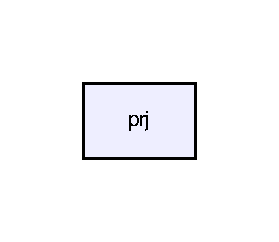
\includegraphics[width=134pt]{dir_47c46492e3b1ef5451c835117c5beee7_dep}
\end{center}
\end{figure}
\subsection*{\-Pliki}
\begin{DoxyCompactItemize}
\item 
plik \hyperlink{main_8cpp}{main.\-cpp}
\begin{DoxyCompactList}\small\item\em \-Plik zawiera glowna funkcje programu. \end{DoxyCompactList}\item 
plik \hyperlink{simplex_8cpp}{simplex.\-cpp}
\begin{DoxyCompactList}\small\item\em \-Definicje poszczegolnych funkcji dla klasy \hyperlink{class_simplex}{\-Simplex}. \end{DoxyCompactList}\item 
plik \hyperlink{simplex_8h}{simplex.\-h}
\begin{DoxyCompactList}\small\item\em \-Plik naglowkowy klasy \hyperlink{class_simplex}{\-Simplex}. \end{DoxyCompactList}\end{DoxyCompactItemize}

\chapter{\-Dokumentacja klas}
\hypertarget{class_simplex}{\section{\-Dokumentacja klasy \-Simplex}
\label{class_simplex}\index{\-Simplex@{\-Simplex}}
}


\-Deklaracja klasy \hyperlink{class_simplex}{\-Simplex}.  




{\ttfamily \#include $<$simplex.\-h$>$}

\subsection*{\-Metody publiczne}
\begin{DoxyCompactItemize}
\item 
\hyperlink{class_simplex_af6f55e322195fb36e8ab68262ec67165}{\-Simplex} (int, int, vector$<$ double $>$, vector$<$ double $>$, vector$<$ vector$<$ double $>$ $>$)
\item 
void \hyperlink{class_simplex_a35bc6fb855df79d43f50c83adee9a564}{\-Oblicz} ()
\item 
double \hyperlink{class_simplex_a62d569cafc5aeb61fa8177cc7301e46f}{\-Max\-Zysk} ()
\item 
double \hyperlink{class_simplex_a6989aacd7767392a9871157a8bd8c67d}{\-Wynik} (int)
\end{DoxyCompactItemize}
\subsection*{\-Atrybuty prywatne}
\begin{DoxyCompactItemize}
\item 
int \hyperlink{class_simplex_a0f6d3ab52d2961e257233c81d4c64c81}{l\-Fabryk}
\item 
int \hyperlink{class_simplex_af05273be3561d707b029894f551bf1fc}{l\-Produktow}
\item 
vector$<$ double $>$ \hyperlink{class_simplex_a3069699ee42dbdb3d94653cefcefd9cc}{zysk\-Produktow}
\item 
vector$<$ double $>$ \hyperlink{class_simplex_a274a651cf1805d25483f1c190d41c0b3}{czasy\-Pracy}
\item 
vector$<$ vector$<$ double $>$ $>$ \hyperlink{class_simplex_a05c1f84eee26b312e4f918016c435a48}{czasy\-Produkcji}
\item 
double \hyperlink{class_simplex_a542e1d670562fb3fa9f11546071c6738}{max\-Zysk}
\item 
vector$<$ double $>$ \hyperlink{class_simplex_a18ae1c3fa2099205b28eb7200c061e9c}{wynik}
\end{DoxyCompactItemize}


\subsection{\-Opis szczegółowy}
\-Deklaracja klasy \hyperlink{class_simplex}{\-Simplex}. 

\-Definicja w linii 17 pliku simplex.\-h.



\subsection{\-Dokumentacja konstruktora i destruktora}
\hypertarget{class_simplex_af6f55e322195fb36e8ab68262ec67165}{\index{\-Simplex@{\-Simplex}!\-Simplex@{\-Simplex}}
\index{\-Simplex@{\-Simplex}!Simplex@{\-Simplex}}
\subsubsection[{\-Simplex}]{\setlength{\rightskip}{0pt plus 5cm}{\bf \-Simplex\-::\-Simplex} (
\begin{DoxyParamCaption}
\item[{int}]{l\-Fabryk, }
\item[{int}]{l\-Produktow, }
\item[{vector$<$ double $>$}]{zysk\-Produktow, }
\item[{vector$<$ double $>$}]{czasy\-Pracy, }
\item[{vector$<$ vector$<$ double $>$ $>$}]{czasy\-Produkcji}
\end{DoxyParamCaption}
)}}\label{class_simplex_af6f55e322195fb36e8ab68262ec67165}


\-Definicja w linii 8 pliku simplex.\-cpp.



\subsection{\-Dokumentacja funkcji składowych}
\hypertarget{class_simplex_a62d569cafc5aeb61fa8177cc7301e46f}{\index{\-Simplex@{\-Simplex}!\-Max\-Zysk@{\-Max\-Zysk}}
\index{\-Max\-Zysk@{\-Max\-Zysk}!Simplex@{\-Simplex}}
\subsubsection[{\-Max\-Zysk}]{\setlength{\rightskip}{0pt plus 5cm}double {\bf \-Simplex\-::\-Max\-Zysk} (
\begin{DoxyParamCaption}
{}
\end{DoxyParamCaption}
)}}\label{class_simplex_a62d569cafc5aeb61fa8177cc7301e46f}


\-Definicja w linii 152 pliku simplex.\-cpp.



\-Oto graf wywoływań tej funkcji\-:\nopagebreak
\begin{figure}[H]
\begin{center}
\leavevmode
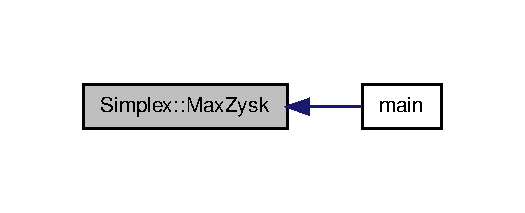
\includegraphics[width=252pt]{class_simplex_a62d569cafc5aeb61fa8177cc7301e46f_icgraph}
\end{center}
\end{figure}


\hypertarget{class_simplex_a35bc6fb855df79d43f50c83adee9a564}{\index{\-Simplex@{\-Simplex}!\-Oblicz@{\-Oblicz}}
\index{\-Oblicz@{\-Oblicz}!Simplex@{\-Simplex}}
\subsubsection[{\-Oblicz}]{\setlength{\rightskip}{0pt plus 5cm}void {\bf \-Simplex\-::\-Oblicz} (
\begin{DoxyParamCaption}
{}
\end{DoxyParamCaption}
)}}\label{class_simplex_a35bc6fb855df79d43f50c83adee9a564}


\-Definicja w linii 22 pliku simplex.\-cpp.



\-Oto graf wywoływań tej funkcji\-:\nopagebreak
\begin{figure}[H]
\begin{center}
\leavevmode
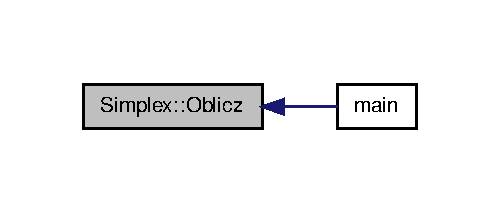
\includegraphics[width=240pt]{class_simplex_a35bc6fb855df79d43f50c83adee9a564_icgraph}
\end{center}
\end{figure}


\hypertarget{class_simplex_a6989aacd7767392a9871157a8bd8c67d}{\index{\-Simplex@{\-Simplex}!\-Wynik@{\-Wynik}}
\index{\-Wynik@{\-Wynik}!Simplex@{\-Simplex}}
\subsubsection[{\-Wynik}]{\setlength{\rightskip}{0pt plus 5cm}double {\bf \-Simplex\-::\-Wynik} (
\begin{DoxyParamCaption}
\item[{int}]{produkt}
\end{DoxyParamCaption}
)}}\label{class_simplex_a6989aacd7767392a9871157a8bd8c67d}


\-Definicja w linii 156 pliku simplex.\-cpp.



\-Oto graf wywoływań tej funkcji\-:\nopagebreak
\begin{figure}[H]
\begin{center}
\leavevmode
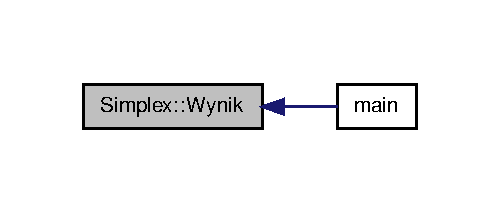
\includegraphics[width=240pt]{class_simplex_a6989aacd7767392a9871157a8bd8c67d_icgraph}
\end{center}
\end{figure}




\subsection{\-Dokumentacja atrybutów składowych}
\hypertarget{class_simplex_a274a651cf1805d25483f1c190d41c0b3}{\index{\-Simplex@{\-Simplex}!czasy\-Pracy@{czasy\-Pracy}}
\index{czasy\-Pracy@{czasy\-Pracy}!Simplex@{\-Simplex}}
\subsubsection[{czasy\-Pracy}]{\setlength{\rightskip}{0pt plus 5cm}vector$<$double$>$ {\bf \-Simplex\-::czasy\-Pracy}\hspace{0.3cm}{\ttfamily  \mbox{[}private\mbox{]}}}}\label{class_simplex_a274a651cf1805d25483f1c190d41c0b3}


\-Definicja w linii 21 pliku simplex.\-h.

\hypertarget{class_simplex_a05c1f84eee26b312e4f918016c435a48}{\index{\-Simplex@{\-Simplex}!czasy\-Produkcji@{czasy\-Produkcji}}
\index{czasy\-Produkcji@{czasy\-Produkcji}!Simplex@{\-Simplex}}
\subsubsection[{czasy\-Produkcji}]{\setlength{\rightskip}{0pt plus 5cm}vector$<$vector$<$double$>$ $>$ {\bf \-Simplex\-::czasy\-Produkcji}\hspace{0.3cm}{\ttfamily  \mbox{[}private\mbox{]}}}}\label{class_simplex_a05c1f84eee26b312e4f918016c435a48}


\-Definicja w linii 22 pliku simplex.\-h.

\hypertarget{class_simplex_a0f6d3ab52d2961e257233c81d4c64c81}{\index{\-Simplex@{\-Simplex}!l\-Fabryk@{l\-Fabryk}}
\index{l\-Fabryk@{l\-Fabryk}!Simplex@{\-Simplex}}
\subsubsection[{l\-Fabryk}]{\setlength{\rightskip}{0pt plus 5cm}int {\bf \-Simplex\-::l\-Fabryk}\hspace{0.3cm}{\ttfamily  \mbox{[}private\mbox{]}}}}\label{class_simplex_a0f6d3ab52d2961e257233c81d4c64c81}


\-Definicja w linii 19 pliku simplex.\-h.

\hypertarget{class_simplex_af05273be3561d707b029894f551bf1fc}{\index{\-Simplex@{\-Simplex}!l\-Produktow@{l\-Produktow}}
\index{l\-Produktow@{l\-Produktow}!Simplex@{\-Simplex}}
\subsubsection[{l\-Produktow}]{\setlength{\rightskip}{0pt plus 5cm}int {\bf \-Simplex\-::l\-Produktow}\hspace{0.3cm}{\ttfamily  \mbox{[}private\mbox{]}}}}\label{class_simplex_af05273be3561d707b029894f551bf1fc}


\-Definicja w linii 19 pliku simplex.\-h.

\hypertarget{class_simplex_a542e1d670562fb3fa9f11546071c6738}{\index{\-Simplex@{\-Simplex}!max\-Zysk@{max\-Zysk}}
\index{max\-Zysk@{max\-Zysk}!Simplex@{\-Simplex}}
\subsubsection[{max\-Zysk}]{\setlength{\rightskip}{0pt plus 5cm}double {\bf \-Simplex\-::max\-Zysk}\hspace{0.3cm}{\ttfamily  \mbox{[}private\mbox{]}}}}\label{class_simplex_a542e1d670562fb3fa9f11546071c6738}


\-Definicja w linii 24 pliku simplex.\-h.

\hypertarget{class_simplex_a18ae1c3fa2099205b28eb7200c061e9c}{\index{\-Simplex@{\-Simplex}!wynik@{wynik}}
\index{wynik@{wynik}!Simplex@{\-Simplex}}
\subsubsection[{wynik}]{\setlength{\rightskip}{0pt plus 5cm}vector$<$double$>$ {\bf \-Simplex\-::wynik}\hspace{0.3cm}{\ttfamily  \mbox{[}private\mbox{]}}}}\label{class_simplex_a18ae1c3fa2099205b28eb7200c061e9c}


\-Definicja w linii 25 pliku simplex.\-h.

\hypertarget{class_simplex_a3069699ee42dbdb3d94653cefcefd9cc}{\index{\-Simplex@{\-Simplex}!zysk\-Produktow@{zysk\-Produktow}}
\index{zysk\-Produktow@{zysk\-Produktow}!Simplex@{\-Simplex}}
\subsubsection[{zysk\-Produktow}]{\setlength{\rightskip}{0pt plus 5cm}vector$<$double$>$ {\bf \-Simplex\-::zysk\-Produktow}\hspace{0.3cm}{\ttfamily  \mbox{[}private\mbox{]}}}}\label{class_simplex_a3069699ee42dbdb3d94653cefcefd9cc}


\-Definicja w linii 20 pliku simplex.\-h.



\-Dokumentacja dla tej klasy została wygenerowana z plików\-:\begin{DoxyCompactItemize}
\item 
\hyperlink{simplex_8h}{simplex.\-h}\item 
\hyperlink{simplex_8cpp}{simplex.\-cpp}\end{DoxyCompactItemize}

\chapter{\-Dokumentacja plików}
\hypertarget{main_8cpp}{\section{\-Dokumentacja pliku /home/martyna/\-Pulpit/calka/prj/main.cpp}
\label{main_8cpp}\index{/home/martyna/\-Pulpit/calka/prj/main.\-cpp@{/home/martyna/\-Pulpit/calka/prj/main.\-cpp}}
}


\-Plik zawiera glowna funkcje programu.  


{\ttfamily \#include $<$iostream$>$}\*
{\ttfamily \#include \char`\"{}integral.\-h\char`\"{}}\*
\-Wykres zależności załączania dla main.\-cpp\-:\nopagebreak
\begin{figure}[H]
\begin{center}
\leavevmode
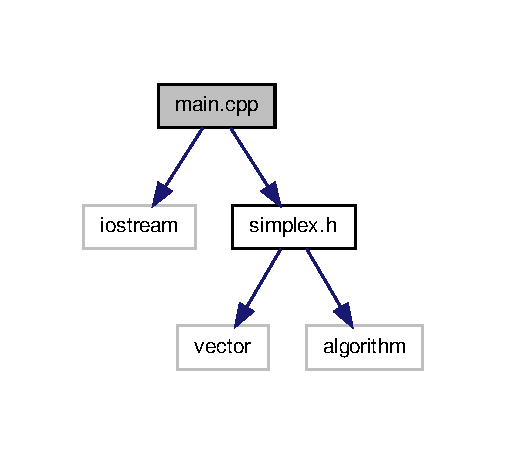
\includegraphics[width=272pt]{main_8cpp__incl}
\end{center}
\end{figure}
\subsection*{\-Funkcje}
\begin{DoxyCompactItemize}
\item 
double \hyperlink{main_8cpp_a80abd7257657e8a5b78f917731d87ba5}{\-F} (double x)
\item 
int \hyperlink{main_8cpp_ae66f6b31b5ad750f1fe042a706a4e3d4}{main} ()
\end{DoxyCompactItemize}


\subsection{\-Opis szczegółowy}
\-Plik zawiera glowna funkcje programu. 

\-Definicja w pliku \hyperlink{main_8cpp_source}{main.\-cpp}.



\subsection{\-Dokumentacja funkcji}
\hypertarget{main_8cpp_a80abd7257657e8a5b78f917731d87ba5}{\index{main.\-cpp@{main.\-cpp}!\-F@{\-F}}
\index{\-F@{\-F}!main.cpp@{main.\-cpp}}
\subsubsection[{\-F}]{\setlength{\rightskip}{0pt plus 5cm}double {\bf \-F} (
\begin{DoxyParamCaption}
\item[{double}]{x}
\end{DoxyParamCaption}
)}}\label{main_8cpp_a80abd7257657e8a5b78f917731d87ba5}


\-Definicja w linii 11 pliku main.\-cpp.



\-Oto graf wywoływań tej funkcji\-:\nopagebreak
\begin{figure}[H]
\begin{center}
\leavevmode
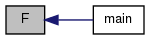
\includegraphics[width=184pt]{main_8cpp_a80abd7257657e8a5b78f917731d87ba5_icgraph}
\end{center}
\end{figure}


\hypertarget{main_8cpp_ae66f6b31b5ad750f1fe042a706a4e3d4}{\index{main.\-cpp@{main.\-cpp}!main@{main}}
\index{main@{main}!main.cpp@{main.\-cpp}}
\subsubsection[{main}]{\setlength{\rightskip}{0pt plus 5cm}int {\bf main} (
\begin{DoxyParamCaption}
{}
\end{DoxyParamCaption}
)}}\label{main_8cpp_ae66f6b31b5ad750f1fe042a706a4e3d4}


\-Definicja w linii 15 pliku main.\-cpp.



\-Oto graf wywołań dla tej funkcji\-:\nopagebreak
\begin{figure}[H]
\begin{center}
\leavevmode
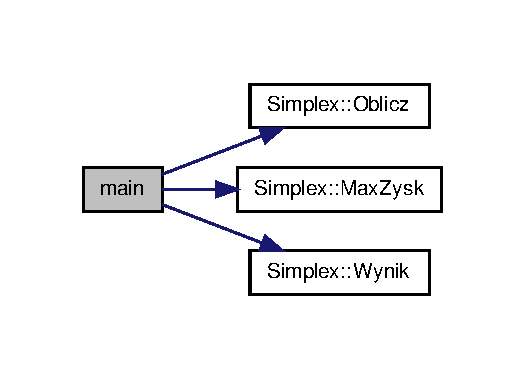
\includegraphics[width=350pt]{main_8cpp_ae66f6b31b5ad750f1fe042a706a4e3d4_cgraph}
\end{center}
\end{figure}



\hypertarget{simplex_8cpp}{\section{\-Dokumentacja pliku simplex.\-cpp}
\label{simplex_8cpp}\index{simplex.\-cpp@{simplex.\-cpp}}
}


\-Definicje poszczegolnych funkcji dla klasy \hyperlink{class_simplex}{\-Simplex}.  


{\ttfamily \#include \char`\"{}simplex.\-h\char`\"{}}\*
\-Wykres zależności załączania dla simplex.\-cpp\-:
\nopagebreak
\begin{figure}[H]
\begin{center}
\leavevmode
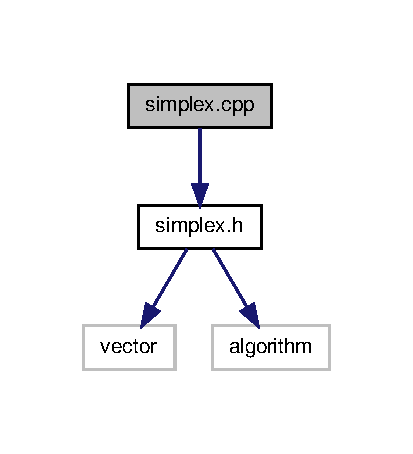
\includegraphics[width=198pt]{simplex_8cpp__incl}
\end{center}
\end{figure}


\subsection{\-Opis szczegółowy}
\-Definicje poszczegolnych funkcji dla klasy \hyperlink{class_simplex}{\-Simplex}. 

\-Definicja w pliku \hyperlink{simplex_8cpp_source}{simplex.\-cpp}.


\hypertarget{simplex_8h}{\section{\-Dokumentacja pliku simplex.\-h}
\label{simplex_8h}\index{simplex.\-h@{simplex.\-h}}
}


\-Plik naglowkowy klasy \hyperlink{class_simplex}{\-Simplex}.  


{\ttfamily \#include $<$vector$>$}\*
{\ttfamily \#include $<$algorithm$>$}\*
\-Wykres zależności załączania dla simplex.\-h\-:
\nopagebreak
\begin{figure}[H]
\begin{center}
\leavevmode
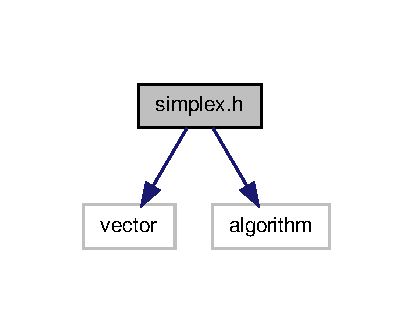
\includegraphics[width=198pt]{simplex_8h__incl}
\end{center}
\end{figure}
\-Ten wykres pokazuje, które pliki bezpośrednio lub pośrednio załączają ten plik\-:
\nopagebreak
\begin{figure}[H]
\begin{center}
\leavevmode
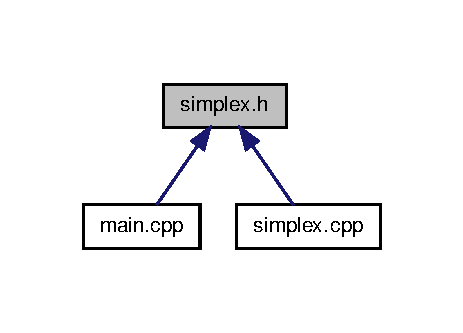
\includegraphics[width=222pt]{simplex_8h__dep__incl}
\end{center}
\end{figure}
\subsection*{\-Komponenty}
\begin{DoxyCompactItemize}
\item 
class \hyperlink{class_simplex}{\-Simplex}
\begin{DoxyCompactList}\small\item\em \-Deklaracja klasy \hyperlink{class_simplex}{\-Simplex}. \end{DoxyCompactList}\end{DoxyCompactItemize}
\subsection*{\-Zmienne}
\begin{DoxyCompactItemize}
\item 
const double \hyperlink{simplex_8h_ad72118df722eee79f65c9f9ef077e909}{\-I\-N\-F} = 1000000000
\end{DoxyCompactItemize}


\subsection{\-Opis szczegółowy}
\-Plik naglowkowy klasy \hyperlink{class_simplex}{\-Simplex}. 

\-Definicja w pliku \hyperlink{simplex_8h_source}{simplex.\-h}.



\subsection{\-Dokumentacja zmiennych}
\hypertarget{simplex_8h_ad72118df722eee79f65c9f9ef077e909}{\index{simplex.\-h@{simplex.\-h}!\-I\-N\-F@{\-I\-N\-F}}
\index{\-I\-N\-F@{\-I\-N\-F}!simplex.h@{simplex.\-h}}
\subsubsection[{\-I\-N\-F}]{\setlength{\rightskip}{0pt plus 5cm}const double {\bf \-I\-N\-F} = 1000000000}}\label{simplex_8h_ad72118df722eee79f65c9f9ef077e909}


\-Definicja w linii 12 pliku simplex.\-h.


\printindex
\end{document}
